\documentclass{article}

\setlength{\parindent}{0pt}
\usepackage{cite}
\usepackage{tikz}
\usepackage{pgflibraryarrows}
\newcommand\independent{\protect\mathpalette{\protect\independenT}{\perp}}
\def\independenT#1#2{\mathrel{\rlap{$#1#2$}\mkern2mu{#1#2}}}



\begin{document}
\section{Implementation}
\subsection{Skeleton}
\subsubsection{Indpendence Test}
The first sprint consisted of implementing the PC algorithm. This began with implementing a function to determine the skeleton of the graph. To estimate the skeleton a function to determine independence and conditional independence of data was needed. The chi squared tests for independence and conditional independence were chosen. This test will only work on discrete data however other tests could be substituted for other data.
\\

Pandas dataframes were chosen to store data during the algorithm as they provide easy indexing and many useful functions. The crosstab function was especially useful when implementing the chi squared tests as it could automatically compute the contingency tables needed for the tests.
\\

A function prepare\_data was implemented to read data from a file into a data frame for processing.\\

The unconditional independence test was fairly straightforward to implement as it only consisted of computing the contingency tables and then comparing the values in the tables to the sums of the rows and columns in the tables.\\

The conditional case was more complex, first the conditioning set was combined into a single variable through concatenation of each variable in every data point. This made making a contingency table across all the observed values significantly easier. Next a contingency table across the three variables was needed. Again the cross tab function was used, however calculating the sums of each time a variable takes a particular value was now more complex, this is because the columns for the conditioning set were split between the columns for the Y variable.\\

On top of this not all values of Y and Z were observed simultaneously in data so
we cant simply iterate through all values of y and z and some up the associated columns as some do not exist. First the columns that exist must be found and then they can be summed over. After this the test is similar to the unconditional however the expected valued will now also account for the value of the conditioning set.
\\

The scipy chi2 function was then used to calculate the chi2 statistic and p-value which is returned by the function.\\

\subsubsection{Variables to be tested}
With this function the skeleton can be found. A fully connected networkx Graph is generated and then edges between nodes that show conditional independence are removed. 

First unconditional independence tests are performed between each pair of variables and edges removed between those that are found to be independent. The conditional tests based on variables adjacent to the first variable with size of the set increasing by one after all tests have been performed. The algorithm tests $X \independent Y | Z$ and $Y \independent X | Z$, this may seem inefficient as it appears that tests are being repeated. However, the members of the set $Z$ are dependent on the first variable in the statement. This means that the tests must all be performed.\\

To find the conditioning sets, the combinations function from the python library itertools was used to find all subsets of $adj(x,G)\ y$ of a certain size.\\

\subsubsection{Order dependence}
The members of set the conditioning set $ Z $ for the test $X \independent Y|Z$ depend on the tests performed before it. This is due to $Z$ consisting of nodes adjacent $X$, however the set of odes adjacent to $X$ changes as edges are removed.\\

In the R implementation an order independent version has been developed. When the size of conditioning sets is incremented, the conditioning sets for all pairs of variables  are calculated and stored. However the original order dependent version can still be used.\\

\subsubsection{Separation sets}
Edge orientation requires the separation set of each pair of variables. This was stored as a dictionary of all pairs of edges and simply updated with a conditioning set if that set was found to condition independence between the pair.\\

Since all of the algorithms learn a skeleton, the function is a method of the GraphLearner class which is the parent class of the other algorithm classes. The function returns a networkx Graph containing the estimated edges of the skeleton and a dictionary containing the separation set of each pair of variables.\\

\subsection{PC edge orientation}
For the pc algorithm edge orientation is relatively simple. However, the pc algorithm outputs a PDAG which contains a mixture of directed and undirected edges, networkx does not contain a data structure to support this kind of graph so one had to be implemented. This turned out to be fairly trivial, using a directed graph behind the scenes in which undirected edges were represented as bidirected edge. Since it's a DAG there cant be any actual bidirected edges so all bidirected edges can simply be considered to be undirected.\\

When finding the edges orientation, one graph was used to store directed and one used to store undirected. When an edge was directed it was simply transferred from one to the other and once all edges that can be oriented are oriented, the two graphs are combined into a PDAG.\\

\subsubsection{V-Structures}
The first part of edge orientation consists of identifying colliders. This is fairly simple as you simply need to find V structures and test if the node that is adjacent to two of the variables is in their separation set. If it is orient the edges toward that node.\\

However, there may be situations in which the order of the v-structures you test affects the final orientation of the graph. There may be two connected v-structures where orienting one will also orient the other but not in the direction described by the constraints.\\

\begin{center}
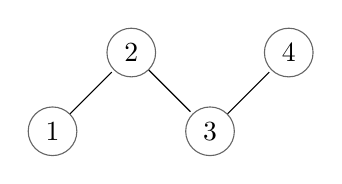
\begin{tikzpicture}[shorten >=1pt,->]
\tikzstyle{vertex}=[circle, draw=black!60, minimum size=12pt]
\node[vertex] (G_1) at (-1,-1) {1};
\node[vertex] (G_2) at (0,0)   {2};
\node[vertex] (G_3) at (1,-1)  {3};
\node[vertex] (G_4) at (2,0)  {4};
\draw [-] (G_1) -- (G_2);
\draw [-] (G_2) -- (G_3);
\draw [-] (G_3) -- (G_4);
\end{tikzpicture}
\end{center}



\begin{center}
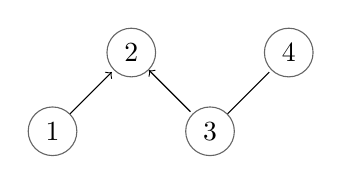
\begin{tikzpicture}[shorten >=1pt,->]
\tikzstyle{vertex}=[circle, draw=black!60, minimum size=12pt]
\node[vertex] (G_1) at (-1,-1) {1};
\node[vertex] (G_2) at (0,0)   {2};
\node[vertex] (G_3) at (1,-1)  {3};
\node[vertex] (G_4) at (2,0)  {4};
\draw [->] (G_1) -- (G_2);
\draw [<-] (G_2) -- (G_3);
\draw [-] (G_3) -- (G_4);
\end{tikzpicture}
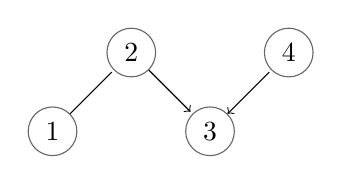
\begin{tikzpicture}[shorten >=1pt,->]
\tikzstyle{vertex}=[circle, draw=black!60, minimum size=12pt]
\node[vertex] (G_1) at (-1,-1) {1};
\node[vertex] (G_2) at (0,0)   {2};
\node[vertex] (G_3) at (1,-1)  {3};
\node[vertex] (G_4) at (2,0)  {4};
\draw [-] (G_1) -- (G_2);
\draw [->] (G_2) -- (G_3);
\draw [<-] (G_3) -- (G_4);
\end{tikzpicture}
\end{center}

Figure - shows two possible orientations, depending on which v structure is oriented first, in the first case when we arrive at the 2,3,4 triple one of two thing can be done. The edge (3,4) can be left undirected or the new structure can override the old one, as shown in figure - .\\

\begin{center}
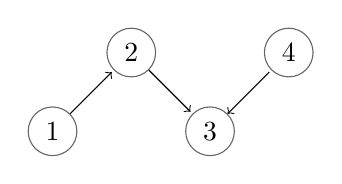
\begin{tikzpicture}[shorten >=1pt,->]
\tikzstyle{vertex}=[circle, draw=black!60, minimum size=12pt]
\node[vertex] (G_1) at (-1,-1) {1};
\node[vertex] (G_2) at (0,0)   {2};
\node[vertex] (G_3) at (1,-1)  {3};
\node[vertex] (G_4) at (2,0)  {4};
\draw [->] (G_1) -- (G_2);
\draw [->] (G_2) -- (G_3);
\draw [<-] (G_3) -- (G_4);
\end{tikzpicture}
\end{center}

In the prexisiting R implementation the second approach of overwriting edges was taken so the same was done in the python implementation.\\

Finally the other orientatian rules described in the algorithm were followed, these were easy to implement using the networkx graphs as they consisted of testing for undirected and directed edges, then orienting based on those tests. This was repeated until no more edges were oriented, this completed the algorithm

\subsubsection{FCI Algorithm}

The FCI algorithm was able to use exactly the same code and first round v-structure orientation of the pc algorithm. However after this code unique to the fci algorithm must be developed.\\

First the final skeleton of the graph must be found. This is done by performing more independence tests, conditioned on the possible d-separating sets of the variables. Finding these sets was made simple by a networkx function to find paths between nodes on a graph.\\

For the rest of the algorithm the network is a PAG. The data structure used for the PAG was a subclass of the networkx undirected graph. In this graph the direction of an edge was determined by tags stored in a dictionary associated with that edge. This allowed all edge types of a PAG to be stored.\\ 




\subsubsection{Testing}

To ensure that the algorithm was behaving as intended all parts must be thoroughly tested. The python unittest module was used to create a test suite covering as many aspects of the algorithm as possible.\\

For the chi squared independence test a sanity check consisting of testing whether a variable was independent of itself was used. Obviously the test will result in a p-value of 0 so was very easy to to test. This test was repeated in the case of a conditioning set of size 1 and size 2 to ensure this did not affect functionality.\\

Next a pre-existing test from r was used to find results on real data. This data was tested with the python implementation and the results compared. Data from the alarm\_10000 and the sia\_1000 datasets were used. Many tests with different variables and conditioning sets were performed.\\

To test the skeleton estimation again the R implementation was used. However, the R version does not use a chi squared test, a wrapper needed to be written to make it compatible with the R skeleton function. With this, skeletons could be generated from data in the same way in python and R and the results compared. The separation sets were also recorded and compared.\\

Testing the edge orientation for the PC algorithm first started with small sanity checks. For example the collider orientation was tested on networks with 3 nodes and two edges and simple separation sets.\\

The path checking needed for the pc algorithm was also  tested on small networks where paths were linear and some with many branches. It was also tested on a few negative examples.\\

Finally a skeleton and separation set generated from the alarms data was oriented in both R and python to test the whole edge orientation process as a whole. However due to the order dependence of the edge orientation the implementations produced slightly different results for the same graphs.\\

This meant that to test the edge orientation section of the pc algorithm, graphs had to be manually oriented using the algorithm and then compared to those estimated by the software.\\

Testing for the FCI algorithm was done in a similar way, however there are many more rules in the FCI algorithm for edge orientation, 10 compared to just 2. To ensure every rule functioned correctly tests were prepared for each rule.\\


\subsection{Final Structure}
The final implementation consisted of four main components. The$\chi^2$ test for independence, the skeleton estimation, PC edge orientation, and FCI edge orientation.\\

\subsubsection{Independence Test}
The $\chi^2$ test was a stand-alone function that can take a data frame along with the names of variables to be tested and a conditioning set. it returns a the $\chi^2$ statistic and a p-value from the test. The p-value represents the probability that the variables are not dependent conditioned on the conditioning set, if this statistic is high enough the variables can be considered independent.

\subsubsection{Graph Learners}
Each algorithm is implemented as a class, the base class of all algorithms is the graph leaner class. These class takes data and an independence test and learn a graph.\\

The base class implements the skeleton learning that all the algorithms use. It can also find and orient colliders on that skeleton. Finally, it has a static method to prepare data, this reads data from a file into a dataframe which can be used by the other methods.\\

The PC algorithm and the FCI algorithms were implemented as subclasses of the Graph learner. The PC algorithm only needed to implement the edge orientation step to complete the algorithm.\\

The FCI algorithm had to both implement edge orientation and extend the skeleton estimation of the graph learner.\\


\subsubsection{Graphs}  
Two new graph classes were implemented, the PDAG and the PAG. The PDAG is a fairly simple extension of networkx's built in Directed graph class in which undirected edges are merely stored as bidirected edges, in PDAGS there are no bidirected edges so ther will be no confusions between bidirected and undirected edges.\\

This implementation is simple but fairly powerful. Most built in networkkx functions will work in a reasonable manner. For example, the has\_edge function will be direction dependent on directed edges but not on undirected edges. Path finding algorithms will also work assuming undiected edges can be tarversed in either direction.\\

\begin{center}
	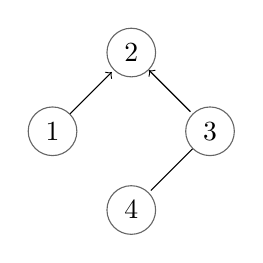
\begin{tikzpicture}[shorten >=1pt,->]
	\tikzstyle{vertex}=[circle, draw=black!60, minimum size=12pt]
	\node[vertex] (G_1) at (-1,-1) {1};
	\node[vertex] (G_2) at (0,0)   {2};
	\node[vertex] (G_3) at (1,-1)  {3};
	\node[vertex] (G_4) at (0,-2)  {4};
	\draw [->] (G_1) -- (G_2);
	\draw [<-] (G_2) -- (G_3);
	\draw [-] (G_3) -- (G_4);
	\end{tikzpicture}
	\quad\quad
	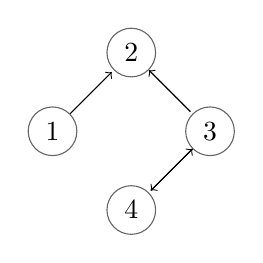
\begin{tikzpicture}[shorten >=1pt,->]
	\tikzstyle{vertex}=[circle, draw=black!60, minimum size=12pt]
	\node[vertex] (G_1) at (-1,-1) {1};
	\node[vertex] (G_2) at (0,0)   {2};
	\node[vertex] (G_3) at (1,-1)  {3};
	\node[vertex] (G_4) at (0,-2)  {4};
	\draw [->] (G_1) -- (G_2);
	\draw [<-] (G_2) -- (G_3);
	\draw [<-] (G_3) -- (G_4);
	\draw [->] (G_3) -- (G_4);
	\end{tikzpicture}
\end{center}

The PAG was more complex to implement due to the increased complexity of the graph. The PAG class is an extension of the undirected graph from networkx. All information about the tags, and therefore the directionality of the edges is stored in an attribute associated with particular edge. The attribute is a dictionary with keys being the nodes at each end of the edge and the values being the tag at that end of the edge.\\

This implementation meant that mayn new methods needed to be added and many existing methods modified. For example, when adding a new edge the tags of the edge needed to be assigned. methods for testing if edges were directed from u to v (had an arrow head into v) or fully directed from u to v (tail at u, arrowhead at v) were created and used during the FCI algorithm.\\

The built in methods for finding paths did however still work with this implementation which was very useful for edge orientation.\\

Currently viewing the graph as a whole is tricky, the built in functions for displaying graphs can not display the edge tags. It may be possible to use the display edge labels function to show the tags as a label on the graph.\\

\begin{center}
	\begin{tikzpicture}[shorten >=1pt,->]
	\tikzstyle{vertex}=[circle, draw=black!60, minimum size=12pt]
	\node[vertex] (G_1) at (-1,-1) {1};
	\node[vertex] (G_2) at (1,1)   {2};
	\node[vertex] (G_3) at (3,-1)  {3};
	\node[vertex] (G_4) at (1,-3)  {4};
	\draw [o->] (G_1) -- (G_2);
	\draw [<-] (G_2) -- (G_3);
	\draw [o-o] (G_3) -- (G_4);
	\end{tikzpicture}
\end{center}
\begin{center}	
	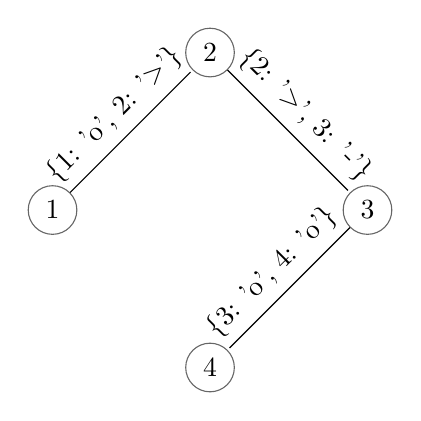
\begin{tikzpicture}[shorten >=1pt,->]
	\tikzstyle{vertex}=[circle, draw=black!60, minimum size=12pt]
	\node[vertex] (G_1) at (-1,-1) {1};
	\node[vertex] (G_2) at (1,1)   {2};
	\node[vertex] (G_3) at (3,-1)  {3};
	\node[vertex] (G_4) at (1,-3)  {4};
	\draw [-] (G_1) -- node[sloped, above]{\{1: 'o', 2: '$>$'\}} (G_2) ;
	\draw [-] (G_2) -- node[sloped, above]{\{2: '$>$', 3: '-'\}} (G_3);
	\draw [-] (G_3) -- node[sloped, above]{\{3: 'o', 4: 'o'\}} (G_4);
	\end{tikzpicture}
\end{center}

\end{document}